\documentclass[12pt]{article}
\usepackage[shortlabels]{enumitem}
\usepackage{graphicx,amsthm}
\begin{document}
\title{TCSS 343 - Week 7}
\author{Jake McKenzie}
\maketitle
\noindent\centerline{\textbf{Homework 5}}
\noindent Do problems 3, 8, 12, 17, 20 from chapter 5.
\noindent 5.3 What is the meaning of the term busy waiting? \\\\
\textbf{ANSWER: }Busy waiting is a method in which a process can do nothing 
until it gets permission to enter its critical section, but continues to execute 
an instruction or set of instructions that tests the appropriate variable to 
gain entrance. \\\\
What other kinds of waiting are there in an operating system? \\\\
\textbf{ANSWER: }
\begin{enumerate}
    \item Sleep: while wasting less cylces than busy waiting, you are
    still wasting cylces. Everytime the thread wakes up it has to 
    reload the thread's stack, registers, and it has to recompute
    if the other thread is done. Also finding the right period to sleep 
    is a non-trivial problem to solve as there are many tradeoffs.
    \item Exponential Backoff: The process of making waiting tasks 
    progressively larger as you wait longer. The analogy for this 
    is waiting for your airplane. If you have half an hour delay 
    you might use the restroom, an hour well then you might play 
    a game on your phone, a few hours and you might read a book.
    \item Locking: You can set up a lock and have the main 
    thread wait on the lock. Then the two threads \textit{notify} 
    when they have finished. Each \textit{notify} wakes the main 
    thread and the main thread check to see if both threads finished.
\end{enumerate}
Can busy waiting be avoided altogether? Explain your answer.\\\\
\textbf{ANSWER: }Busy waiting cannot be avoid because not all processes 
are created equal and are best tracked using busy waiting as opposed to 
the alternatives above. The alternative methods above work best 
on smaller embedded devices with real time operating systems, but as 
you start getting into multiprocessors it becomes harder and harder to avoid 
busy waiting. \\\\
5.8 The first known correct software solution to the critical-section problem
for two processes was developed by Dekker. The two processes, P0 and
P1, share the following variables:\\
\centerline{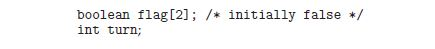
\includegraphics[scale = 1]{code2.jpg}}\\
The structure of process Pi (i == 0 or 1) is shown in Figure 5.21. The
other process is Pj (j == 1 or 0). Prove that the algorithm satisfies all
three requirements for the critical-section problem.\\\\
\textbf{ANSWER: }
\begin{proof} Mutual exclusion is enforced if a process is executing in 
it's critical section, then no other process can execute in its own 
critical section. This is enforced with flags. One way that this can be proven
true is by adding the line assert(flag[i]\&!flag[j]) or 
the statement assert(flag[j]\&!flag[i]). At no stage in Dekkar's 
algorithm is this false so the assert never fires.
\end{proof}
\begin{proof}
    Progress is enforced when no progress is in a ciritcal section, any process
    that requests entry to the critical section must be permitted to enter without
    delay. No starvation means there is an upper bound on the number of processes 
    that can enter it's critical sections while another is waiting.
    Consider $P_i$ is attempting to enter the cirtical section. 
    Since only one process is trying to enter the critical section, flag[j] will 
    will be false. So the process enters the critical section without difficulty.
    Now consider that $P_i$ and $P_j$ are attempting to enter their critical section, 
    and their turn = 0. The value of turn is modified only after one process has exited 
    its critical section, since both processes enter the loop.
    If flag[i] = false, $P_j$ checks flag[i] and finds it is false. So $P_j$ enters the 
    critical section immediately.  
    If flag[j] = true, since turn = 0, the proces $P_i$ will wait in its external loop for 
    flag[j] to be set to false. This is where $P_i$ enters the critical section. Both progress 
    and no starvation are satisfied.
\end{proof}
5.12 The Linux kernel has a policy that a process cannot hold a spinlock while
attempting to acquire a semaphore. Explain why this policy is in place.\\\\
\textbf{ANSWER: } In linux you cannot sleep while holding a spinlock and you have to 
sleep while waiting for the semaphore. In other words, spinlocks are used in an interrupt 
context, where sleeping is not allowed while semaphores are used in a process context, 
where sleeping is okay.\\\\
5.17 Assume that a system has multiple processing cores. For each of the
following scenarios, describe which is a better locking mechanism—a
spinlock or a mutex lock where waiting processes sleep while waiting
for the lock to become available:\\\\
• The lock is to be held for a short duration.\\
\textbf{ANSWER: }Mutex's can cause context switches while spinlocks cannot, making 
them ideal for processes held for short durations.\\\\
• The lock is to be held for a long duration.\\
\textbf{ANSWER: }Since mutex's enforce a serial queue, this makes them ideal for thread 
equity. In the aggregate this allows the rest of the processing cores to schedule 
other processes while locked processes wait, not allowing this behaivor performing worse 
than spinlocks.\\\\
• A thread may be put to sleep while holding the lock.\\
\textbf{ANSWER: }A mutex lock is required as you do not want the waiting process to be 
spinning while waiting for the other process to wake up.\\\\
5.20 Consider the code example for allocating and releasing processes shown
in Figure 5.23.\\\\
\textbf{ANSWER: }Since the number\_of\_processes can become greater than the MAX\_PROCESSES if
multiple instances are running this causes a race condition ++number of processes; line and 
the line with --number of processes;.
2. From the following code, answer these questions:\\\\
a- whate is the role of the\_mutex?\\\\
\textbf{ANSWER: }The role of the\_mutex is to provide a \textit{lock} by providing mutual 
exclusion for the shared data. It accomplishes this by protecting the buffer and releasing 
the buffer when the consumer is ready.\\\\
b- What is the role of condition variable condp?\\\\
\textbf{ANSWER: }This condition is met when it is time to put information into the buffer.\\\\
c- What is the role of condition variable condc?\\\\
\textbf{ANSWER: }This condition is met when it is time to take information into the buffer.\\\\
d- Why there is a while loop in lines a and b instead of a simple if
statement?\\\\
\textbf{ANSWER: } We need to break from the loop if the condition of the while loop 
is met to ensure mutual exclusion for the monitor. The if statement, while doing 
the action of what we want allows for the buffer to overflow.\\\\
e- What is the NULL for in line c? Which parameter is affected?\\\\
\textbf{ANSWER: }In this line of code we are setting the lock to NULL so that we 
can kill the \textit{lock}.\\\\
\end{document}